\documentclass[letterpaper, 10 pt, conference]{ieeeconf}  % Comment this line out if you need a4paper
%\documentclass[a4paper, 10pt, conference]{ieeeconf}      % Use this line for a4 paper
\IEEEoverridecommandlockouts                              % This command is only needed if 
                                                          % you want to use the \thanks command
\overrideIEEEmargins                                      % Needed to meet printer requirements.

\usepackage[pdftex]{graphicx}
\usepackage{algpseudocode}
\usepackage{subfigure}
\usepackage[noadjust]{cite}

\title{\LARGE \bf
  % Longitudinal Trajectory Planning and Tracking for Fixed-Path Autonomous Driving
  % Reactive Path Planning with Pedestrains for Autonomous Driving
  Reactive Trajectory Planning and Trajectory Tracking for Pedestrian-Aware Autonomous Driving in Urban Environments
}

\author{
  Robert G. Cofield $^{1}$ and
  Rakesh Gupta $^{2}$
  \thanks{
    * This work was performed at Honda Research Institute USA.
  }
  \thanks{
    $^{1}$ Auburn University GAVLab, 1418 Wiggins Hall, Auburn, AL 36832. \textit{robertgcofield@gmail.com}
  }
  \thanks{
    $^{2}$ Honda Research Institute USA Inc, 375 Ravendale Drive, Mountain View, CA 94043. \textit{rgupta@hra.com}
  }
}

%%%%%%%%%%%%%%%%%%%%%%%%%%%%%%%%%%%%%%%%%%%%%%%%%%%%%%%%%%%%%%%%%%%%%%%%%%%%%%%%
%%%%%%%%%%%%%%%%%%%%%%%%%%%%%%%%%%%%%%%%%%%%%%%%%%%%%%%%%%%%%%%%%%%%%%%%%%%%%%%%
%%%%%%%%%%%%%%%%%%%%%%%%%%%%%%%%%%%%%%%%%%%%%%%%%%%%%%%%%%%%%%%%%%%%%%%%%%%%%%%%

\begin{document}

\maketitle
\thispagestyle{empty}
\pagestyle{empty}

%%%%%%%%%%%%%%%%%%%%%%%%%%%%%%%%%%%%%%%%%%%%%%%%%%%%%%%%%%%%%%%%%%%%%%%%%%%%%%%%
\begin{abstract}

In this paper, we address the problem of trajectory planning for urban roads while reacting to the presence of pedestrians.
Past work reduces jerk and limits velocities and acceleration to smooth trajectories, but it does not consider reactive behaviors such as responding to pedestrians.
On the other hand, systems for collision avoidance plan paths around obstacles and pedestrians, stop for them, or produce a warning. 
In this paper, we present an integrated trajectory generation and tracking system for urban environments that simultaneously considers constraints to maximize human comfort and real-time trajectory updates to react to pedestrians on the road. 

Given a desired path, we present a novel online method for planning longitudinal trajectories to follow the urban path with turns and intersections while honoring traffic regulations such as stop signs.
Based on sensor data, our method updates the trajectory plan to safely avoid pedestrians on the road by slowing or stopping.
This is critical in urban environments, when modifying the vehicle's intended path is often not possible.
Our method has closed form solutions, runs at 20 Hz, and is efficient and reliable for use in online planning.
We have confirmed this with a test vehicle and pedestrians with over 100 hours of testing under driverless operation.

\end{abstract}
%%%%%%%%%%%%%%%%%%%%%%%%%%%%%%%%%%%%%%%%%%%%%%%%%%%%%%%%%%%%%%%%%%%%%%%%%%%%%%%%

%%%%%%%%%%%%%%%%%%%%%%%%%%%%%%%%%%%%%%%%%%%%%%%%%%%%%%%%%%%%%%%%%%%%%%%%%%%%%%%%
\section{Introduction} \label{sec:introduction}

When planning trajectories for an autonomous ground vehicle operating on roadways, a typical goal is to minimize navigation time.
It is common to employ the path-velocity decomposition to separate the two tasks so that they can be carried out sequentially or in parallel.
% (i.e., path planning is performed prior to planning the speed that the vehicle will take along the chosen path).
First is Path Planning, which involves computation of the optimal path.
The second task is Trajectory Planning, which involves the computation of the fastest velocity profile that is appropriate for the scenario.

Computation of a trajectory plan for traveling from one point to another is often guided by
passenger comfort. The set of possible paths to the destination is typically restricted 
by constraints such as traversability and legally available travel lanes, among others.
The intended speed, acceleration, and higher derivatives of position with respect to time are also subject to constraints.
These include legal speed limits, engine dynamics, desired side-slip limits, traction availability, and rollover concerns.

For human passengers, it is widely believed that high levels of jerk (time derivative of acceleration) and high acceleration/velocity values are prime contributors to ride discomfort.
A lot of work has been performed on optimizing these constraints for highways and country roads ~\cite{ziegler14,bahram15,xu12,CHEB15CI}.
Some preliminary work on optimizing these constraints on urban roads has been done ~\cite{Rastelli14,Li15} but they do not consider reactive behavior such as responding to pedestrians or other dynamic objects in the scene.
On the other hand, many systems in the literature find and plan paths around pedestrians, stop for them, or produce a warning ~\cite{pradalier05,benenson06,gu14,mogelmose15,johnson13} but do not work as part of an integrated system that can navigate urban roads.
In this paper, we describe an trajectory generation system that satisfies these constraints for human comfort and is reactive to presence of pedestrians on the road.
%Some work has been done for reacting to pedestrians such as by Singapore groups but it has been done at very low speeds (5 miles/hour).
%There has also been some work in simulating vehicles and modeling uncertainty, but pedestrians are less predictable than cars 
%and can appear suddenly on the road (when someone is jaywalking for example).

In this paper, we present an autonomy framework for pedestrian aware ground vehicles.
Our objective is to travel autonomously from start to destination while honoring traffic laws and avoiding pedestrians on the roadway.
%Desired behavior from the car includes following traffic laws at the intersections such as stop signs.
At stop signs the car should stop and wait for an appropriate amount of time.
It should also react to pedestrians on the road - at intersections as well as on the road.
Pedestrians on the sidewalks should be ignored by the autonomous cars.
Further the pedestrians can be static or moving.
The car should stop, slow down and circum-navigate around pedestrians when appropriate.

Given a desired path, we present a novel method for planning longitudinal trajectories (i.e., the time derivatives of position in the body-forward direction) along that path.
Our method first segments the path using an arbitrary set of kinematic or dynamic constraints which may be functions of the desired path.
Each segment is then planned sequentially by choosing a piecewise constant jerk profile.
The jerk profile is intelligently chosen from a set of pre-solved profiles such that acceleration is continuous and non-infinite throughout the entire path.
The resultant trajectory plan can then be easily sampled to provide a reference for real-time vehicle control, which is called trajectory tracking control.
We present an online method of revising the trajectory plan to safely avoid pedestrians that enter the roadway by slowing or stopping when no alternative paths are available.

We first describe the architecture of our system in Sec. \ref{sec:systemarchirecture}.
We also describe other subsystems that our system needs to work with, and planned stops.
In Section \ref{sec:trajectoryplanning}, we describe trajectory planning which takes a 2D path and generates a trajectory that satisfies jerk and maximum velocity and acceleration constraints. 
We explain how we handle intersections, turns in the road and planned stops due to stop signs (that have already been marked in the map).
We then describe extensions to trajectory planner that handle reactivity to pedestrians in the environment. 
Once a trajectory plan is formulated, it must be utilized online to send the reference signal to the controllers that govern steering, braking, and engine speed.
This is the trajectory tracking problem, which is discussed in Section \ref{sec:trajectorytracking}.
Section V describes the high level Path Manager that calls the trajectory planner as necessary to 
exhibit reactionary behavior and stop for pedestrians that may appear on the road.
We then conclude and discuss future extensions.
% tracking

%%%%%%%%%%%%%%%%%%%%%%%%%%%%%%%%%%%%%%%%%%%%%%%%%%%%%%%%%%%%%%%%%%%%%%%%%%%%%%%%
%%%%%%%%%%%%%%%%%%%%%%%%%%%%%%%%%%%%%%%%%%%%%%%%%%%%%%%%%%%%%%%%%%%%%%%%%%%%%%%%

\section{System Architecture} \label{sec:systemarchirecture}

Our system architecture is shown in Figure \ref{fig:addreact}.
There are 4 primary input components: a path planner, navigation filter, pedestrian detector, and a map which provides the location of stop signs.
% nav filter
For navigation filtering we use an ADMA-G  commercial automotive GPS/INS system.
It receives RTK corrections via cell modem.
It outputs global position, global heading, body frame velocity and body frame acceleration to centimeter level accuracy.

\begin{figure}[thpb]
  \centering
  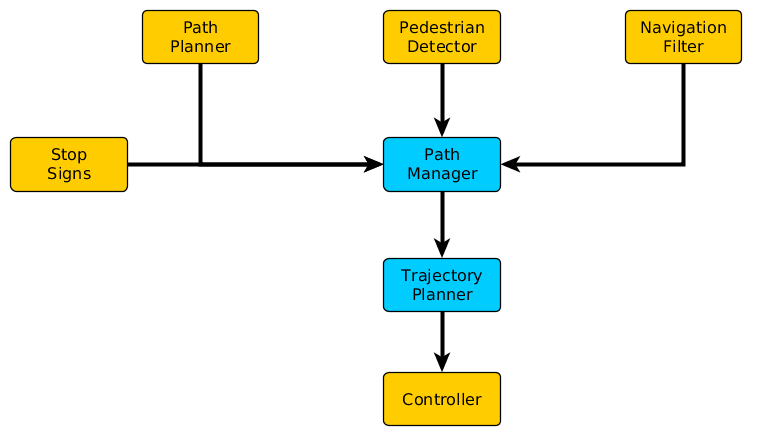
\includegraphics[width=1.0\columnwidth]{graphics/MissingReactionPiece2.png}
  \caption{
   Primary system components. The ``Path Manager'' and ``Trajectory Planner'' scomponents (in blue) are presented herein.
  }
  \label{fig:addreact}
\end{figure}

Pedestrian detection is performed via a camera and LiDAR system based on \cite{Gepperth2013,Gepperth2014}.
It computes a bounding box for each pedestrian as shown in Figure \ref{fig:ped}.
The pedestrian position is transformed to the vehicle body frame, and subsequently transformed to global frame to be related to the planned path.

\begin{figure}[thpb]
  \centering
  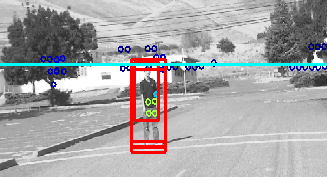
\includegraphics[width=0.5\columnwidth]{graphics/ped3.png}
  \caption{Showing detected pedestrian by the computer vision system
  \newline
  }
  \label{fig:ped}
\end{figure}

We assume that we have access to a path planner.
For example, this can be a service similar to Google Maps except that it provides lane level maps. 
We assume that the path planner operates independently from the trajectory planner and tracker.
We also assume that we have a high resolution digital map with lane centers, stop signs, crosswalk geometry, and turning curves at intersections.
The destination is manually input into the system by the passengers.
Using the path planner, we obtain a path along lane centers from the vehicle's current location (computed by the navigation filter) to the destination.
This plan is output as set of global waypoints, with the waypoints corresponding to stop signs flagged.
This same map database is used to search for stop signs and provide their locations.

%\begin{figure}[thpb]
%  \centering
%  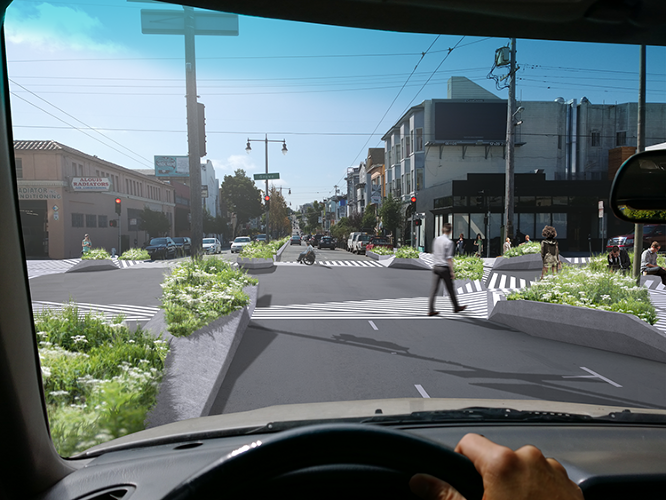
\includegraphics[width=1.0\columnwidth]{graphics/3023096-slide-c4carafter.png}
%  \caption{Pedestrain at the intersection}
%  \label{fig:ped2}
%\end{figure}

\begin{figure}[thpb]
  \centering
  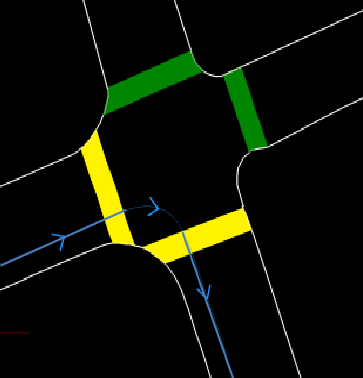
\includegraphics[width=0.3\columnwidth]{graphics/IntersectionCrosswalks.png}
  \caption{
    A car turning right at the intersection only needs to consider pedestrians in the pedestrian crossings shown yellow.
    Pedestrians in the green crossings can be ignored unless they appear somewhere on the road.
  }
  \label{fig:intersect}
\end{figure}

We also have an In-Out Algorithm implemented via polygon intersection that can be used to ignore “safe” pedestrians
Pedestrians that are on sidewalks, off-path crosswalks, and behind planned stops as shown in Figure \ref{fig:intersect} can be considered ``safe'' and are ignored.
This is done by searching the same map database used for path planning.
Remaining pedestrians pose collision risk and the vehicle needs to reactively slow down or stop for them.
This is accomplished by sending stop message with pedestrian locations to the path manager.

Beyond the input subsystems, there are three other major components: a high-level planner, a low-level planner, and a software controller which governs engine speed, braking, and steering.
The controller takes as an input a trajectory which is sampled at 10 Hz and spans 2 seconds, beginning at the moment of data transmission.
This short-term trajectory is oriented in the vehicle body frame.
\textbf{Citation for controller ????}.

The high-level planner is referred to as the ``path manager'', and performs decision-making as well as governing operation of the low-level planner.
Its primary functions are:
\begin{enumerate}
  \item Stop the vehicle at stop signs and wait until the assosciated intersection is clear before continuing.
  \item Reactively reduce speed or stop altogether for pedestrians which pose a collision risk, then continue when they are clear.
  \item Govern the trajectory planner.
\end{enumerate}
The low-level planner is referred to as the ``trajectory planner'', and is responsible for quantifying the actions dictated by the path manager.
Its primary functions are:
\begin{itemize}
  \item Compute medium-range trajectories for a given path.
  \item Revise trajectories to react to pedestrians.
  \item Sample the current trajectory for input to the controller.
\end{itemize}
This work focuses on the path manager (Sec. \ref{sec:pathmanager}) and the trajectory planner (Sec. \ref{sec:trajectoryplanning} \& Sec. \ref{sec:trajectorytracking}).

%%%%%%%%%%%%%%%%%%%%%%%%%%%%%%%%%%%%%%%%%%%%%%%%%%%%%%%%%%%%%%%%%%%%%%%%%%%%%%%%
%%%%%%%%%%%%%%%%%%%%%%%%%%%%%%%%%%%%%%%%%%%%%%%%%%%%%%%%%%%%%%%%%%%%%%%%%%%%%%%%

\section{Path Manager} \label{sec:pathmanager}

The path manager is implemented as a discrete state machine, depicted in Fig. \ref{fig:st}.
Each of the states is described below.


\begin{figure}[thpb]
  \centering
  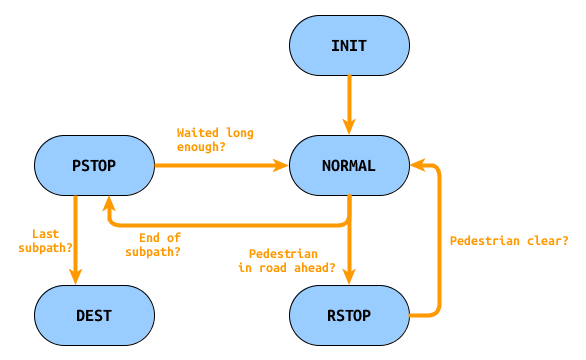
\includegraphics[width=1.0\columnwidth]{graphics/StateMachineSimple.png}
  \caption{State Transition Diagram}
  \label{fig:st}
\end{figure}

Many systems perform trajectory planning over a sliding window within the full path which progresses with the vehicle.
This requires ... \textbf{something about computing actions through stop signs before it's necessary and how that's inefficient}.
We propose to break the path into sub-paths at each stop location which is known a priori, as shown in Fig. \ref{fig:segmentation}, and  execute them incrementally.

In the absence of pedestrians, the path manager cycles between PSTOP and NORMAL states.
In NORMAL state, the path manager send the first subpath to the trajectory planner, which then plans and executes it before coming to a stop at the end of the subpath.
In PSTOP mode, the path manager waits for a pre-set time duration before returning to NORMAL mode, where the next subpath is executed.
When pedestrians are present, the transition from PSTOP to NORMAL is delayed until there are no pedestrians detected in the range denoted by $\Delta s_{resume}$.

\begin{figure}[thpb]
  \centering
  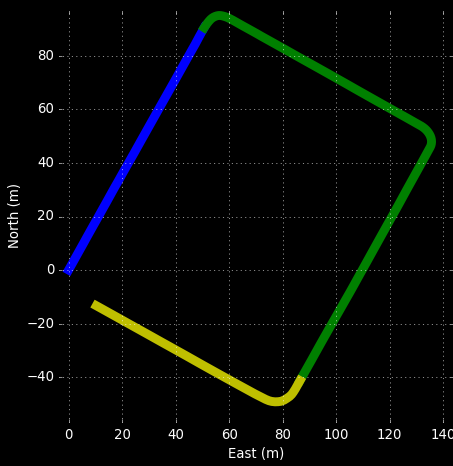
\includegraphics[width=0.5\columnwidth]{graphics/Subpaths.png}
  \caption{
    Segmentation of the path by path manager.
    The trajectory generation is serially called on each segment colored differently.
  }
  \label{fig:segmentation}
\end{figure}

All detected pedestrians locations are compared against the high-resolution digital map, so that pedestrians which are not on the roadway or near an upcoming crosswalk are not considered.
Then each pedestrian location is projected onto the total path in the same manner as described in Sec. \ref{sec:trajectorytracking}.
Pedestrians which are on a different subpath than the vehicle are disregarded, as well as those which are behind the vehicle (i.e., $s_{ped} < s_{veh}$).
All the pedestrians which remain pose a potential collision risk, however only the closest is considered for RSTOP.

The distinction between momentarily braking for a pedestrian which quickly leaves the roadway and coming to a full stop needs no formal logic.
They follow the same state transition, and since all trajectory plans are extremely smooth, riders are rarely aware that any change took place.
It should be noted that there is a brief waiting period before resuming NORMAL mode from RSTOP to ensure that no tracking errors occurred in the pedestrian detection algorithm.

\begin{figure}[thpb]
\centering
  \subfigure[In NORMAL mode, RSTOP is now triggered.]{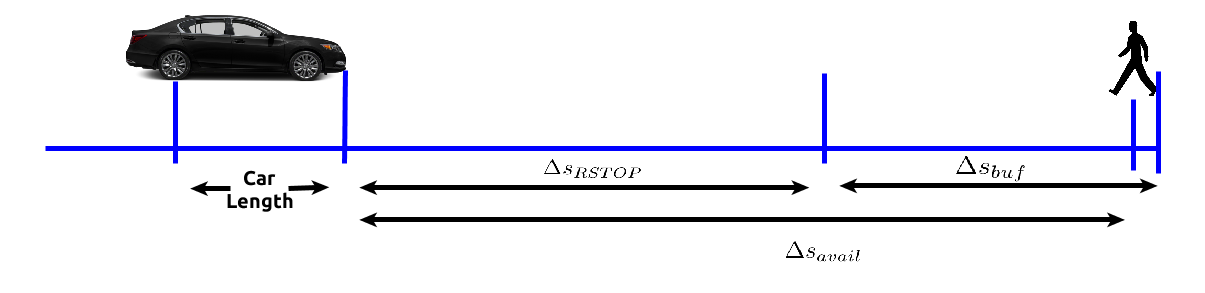
\includegraphics[width=1.0\columnwidth]{graphics/RSTOP_NORMAL_time_to_stop.png}}
  \\
  \subfigure[RSTOP diagram showing bounds for revising the RSTOP trajectory.]{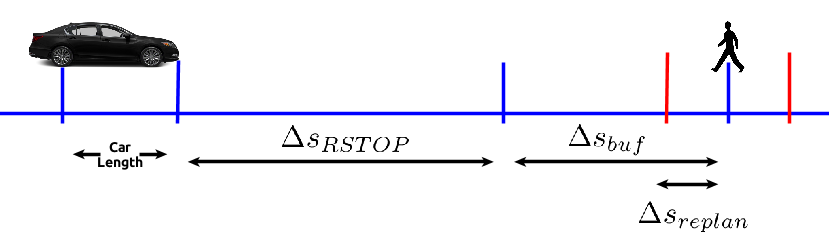
\includegraphics[width=1.0\columnwidth]{graphics/RSTOP_Replan.png}}
  \\
  \subfigure[PSTOP diagram showing bounds for reverting to NORMAL mode.]{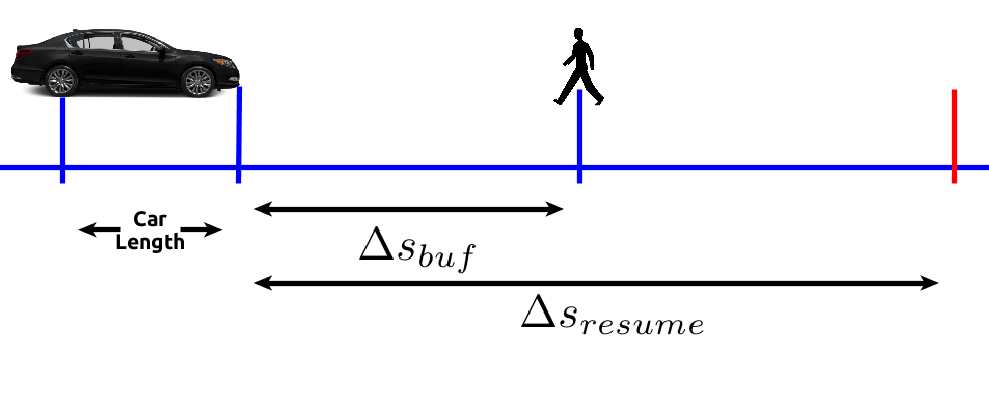
\includegraphics[width=1.0\columnwidth]{graphics/RSTOP_Resume.png}}
  \caption{Graphical representation of static and dynamic thresholds used to trigger state transitions.}
  \label{fig:react}
\end{figure}

Next the nominal distance needed to stop $\Delta s_{RSTOP}$ must be computed given the vehicle's current location, speed, and forward acceleration.
The procedure for doing this will be the same as the procedure for planning the RSTOP trajectory later with a few steps omitted, since the planning algorithm is extremely efficient.

Note that a static buffer distance, $\Delta s_{buf}$ is added to ensure safety and comfort.
RSTOP is triggered when $\Delta s_{RSTOP} + \Delta s_{buf} >= s_{ped} - s_{veh}$ and the actual available stopping distance $\Delta s_{avail} = s_{ped} - s_{veh}$ is computed.
Planning and executing the trajectory for coming to a halt is detailed in Sec. \ref{sec:reactivestoptrajectory}.

This procedure is repeated when the nearest pedestrian location changes by a value more than some static buffer $\Delta s_{replan} < \Delta s_{buf}$ compared to the location for which the current RSTOP planned.
This value is typically set to 1 meter.
Normal operation is resumed when the distance between the vehicle and the closest detected pedestrian satisfies $s_{ped} - s_{veh} > \Delta s_{resume} + \Delta s_{RSTOP}$. The static resume buffer should be set such that $\Delta s_{resume} > \Delta s_{buf} + \Delta s_{replan}$.
The preceding quantities are depicted graphically in Fig. \ref{fig:react}.

%%%%%%%%%%%%%%%%%%%%%%%%%%%%%%%%%%%%%%%%%%%%%%%%%%%%%%%%%%%%%%%%%%%%%%%%%%%%%%%%
%%%%%%%%%%%%%%%%%%%%%%%%%%%%%%%%%%%%%%%%%%%%%%%%%%%%%%%%%%%%%%%%%%%%%%%%%%%%%%%%

\section{Trajectory Planning} \label{sec:trajectoryplanning}

The task trajectory planning in this context is to take a 2 dimensional (horizontal plane) set of waypoints from the path manager, and compute a series of constant jerk intervals for motion along the length of the path.
This trajectory must be time optimal yet still fall within constraints on speed, acceleration, and jerk.
Elevation changes will not be addressed here.
Integrating piecewise constant jerk over time yields acceleration which is piecewise linear over time, speed which is piecewise quadratic over time, and position which is piecewise cubic over time.

Prescribed initial and end conditions for position, speed, and acceleration must also be honored.
This means that the desired trajectory plan may be mapped into one dimension using curvilinear coordinates to significantly simplify the solution.
We show how two dimensional concerns (specifically cornering speeds for this work) are expressed in one dimension to guide planning.
All planning is longitudinal; that is, speed is the primary focus, and we assume that the control subsystem will ensure that the vehicle follows the prescribed path.

\begin{figure}[thpb]
  \centering
  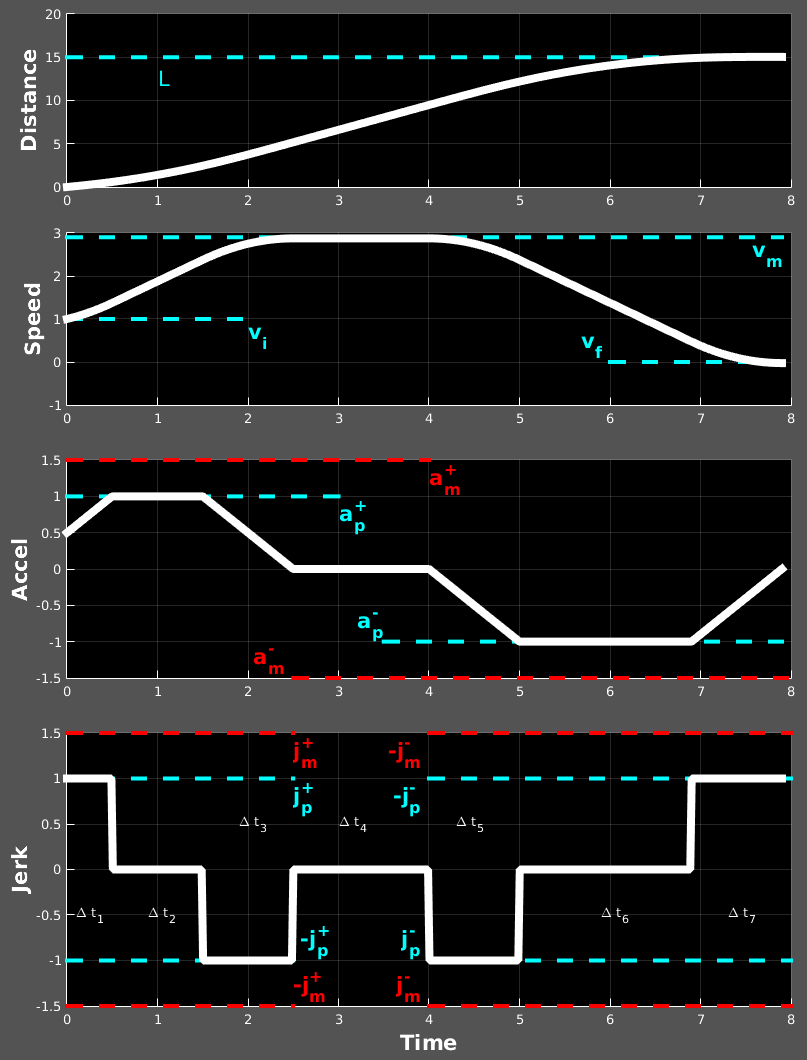
\includegraphics[width=1.0\columnwidth]{graphics/Full7PhaseSpecVertical.png}
  \caption{
    7 phase constant jerk profile along curvilinear distance axis.
    All values needed to completely parameterize a single path segment for trajectory are labeled here.}
  \label{fig:full7phasespec}
\end{figure}

%%%%%%%%%%%%%%%%%%%%%%%%%%%%%%%%%%%%%%%%%%%%%%%%%%%%%%%%%%%%%%%%%%%%%%%%%%%%%%%%

\subsection{Jerk Profiles} \label{sec:jerkprofiles}

Consider, as a starting point, the case in which a vehicle is moving at some small initial speed and needs to accelerate to some traveling speed, maintain that speed for some distance, then brake to a stop at a prescribed end location.
Figure \ref{fig:full7phasespec} shows this trajectory over time.
The problem is defined by the vector of known values $\mathbf{b}  = [v_i, a_i, L, v_m, v_f]$, being initial speed, initial acceleration, the total distance, speed limit, and the final speed, respectively.
It is assumed that the final forward acceleration will be zero.
If the magnitude of the desired peak acceleration and jerk ($a_m$ and $j_m$, respectively) are known, then a profile with $M$ jerk phases (7 in this case) can be generated by solving for the time intervals $[\Delta t_1, ..., \Delta t_M]$.
Jerk and peak acceleration may be different when reducing speed versus increasing speed to more closely mirror human driving behavior \emph{Citation}.
The remaining parameters yet to be set now become $\mathbf{a}_m = [a^+_m , a^-_m]$ and $\mathbf{j}_m = [j^+_m , j^-_m]$.
As we show later, peak acceleration and jerk must sometimes be modified to obtain physically possible time intervals.
To enable this, ranges of acceptable longitudinal jerk and acceleration $\mathbf{a}^{max}_m = [a^{+,max}_m , a^{-,max}_m]$ and $\mathbf{j}^{max}_m = [j^{+,max}_m , j^{-,max}_m]$ are set according to the relation in Eqs. \ref{eq:am} and \ref{eq:jm}.
This is computed for every point along the path.
In the simplest case, one value for each of the quantities expressed in these relations may be chosen for the entire path.

\begin{equation}
  a^{+,max}_m >= a^+_m > 0 > a^-_m >= a^{-,max}_m
  \label{eq:am}
\end{equation}
\begin{equation}
  j^{+,max}_m >= j^+_m > 0 > j^-_m >= j^{-,max}_m
  \label{eq:jm}
\end{equation}

There are many cases in which this solution will fail.
For instance, if $L$ is sufficiently short and $v_m$ is sufficiently high, then it will not be possible to ever reach $v_m$ with realistic values of $\mathbf{a}_m$ and $\mathbf{j}_m$.
We propose to define 4 other basic profiles, and our algorithm judiciously chooses the appropriate profile for every segment defined by a vector $\mathbf{b}$.
The other profiles are explained below in Section \ref{sec:jerkprofiles}.
A path is then a set of $N_s$ segments, each of which is defined by a set of parameters $\mathbf{b}_k, k = 1 ... N_s$ and can be solved individually in sequence.
Determination of where to break a path into segments is discussed below in Section \ref{sec:pathsegmentation}.

There are a total of five potential jerk profiles which have been created to cover all feasible values in $\mathbf{b}$.
All impossible scenarios are automatically ruled out (e.g., end speed above speed limit, traveling speed of zero, negative speeds in $\mathbf{b}$, etc).
It should be noted that traveling backward (i.e., in reverse gear) is not supported in this work.
To find closed-form solutions for each, a symbolic solver was used.
The target values for each profile are the time steps between jerk changes.
These are solved by plugging in $\mathbf{b}$, $\mathbf{a}_m$, and $\mathbf{j}_m$.

For each of the profiles, it is possible that the chosen values of $\mathbf{a}_m$ and $\mathbf{j}_m$ will not be feasible for a desired speed at the end of the phase.
This results in a negative time interval for that phase.
In many cases, modifying $\mathbf{a}_m$ and $\mathbf{j}_m$ such that they still lie within $\mathbf{a}^{max}_m$ and $\mathbf{j}^{max}_m$ will remedy this.
Specifically, jerk may be increased while peak acceleration is decreased.
This process is referred to herein as ``accel-jerk tuning''
If no acceptable values are found within the valid ranges of $\mathbf{a}^{max}_m$ and $\mathbf{j}^{max}_m$, a new jerk profile must be chosen.

To decide which profile to employ, a cascade approach is used.
Analytic values of time intervals are evaluated for each profile by plugging in values of $\mathbf{b}$, $\mathbf{a}_m$, and $\mathbf{j}_m$ until all time intervals are positive and real.
The order in which they are attempted is: 7 $\rightarrow$ 6 $\rightarrow$ 4 / 4R $\rightarrow$ 3.

\subsubsection{7 Phase} \label{sec:7phase}

This profile, with $\Delta t_i$ as shown in Figure {fig:full7phasespec}, is always attempted first.
All time steps have a single solution, enabled by the fact that the initial and end conditions are known, and the two peak accelerations and two jerk magnitudes are provided as configuration parameters.
In the case where $\Delta t_2$ or $\Delta t_6$ are negative, accel-jerk tuning must be employed.
In the instance where $\Delta t_4$ is negative, the total segment length $L$ is too short to reach top speed of $v_m$, so a 6 phase profile must be used.

\subsubsection{6 Phase} \label{sec:6phase}

In the case mentioned above, the speed limit is too high for a solution to exist for a 7 phase profile.
The middle travel period $\Delta t_4$ is removed, so that the vehicle increases speed and then immediately decreases speed. 
The peak speed in this case has a solution, but cannot be manipulated directly.
Without this known value, the problem becomes under-defined, so $\Delta t_2$ and $\Delta t_5$ each have two solutions: one negative and one positive.
The positive solution is chosen.
In the case where both solutions are negative, accel-jerk tuning is attempted. 
Should that yield no positive time intervals, one of the two 4 phase profiles then becomes appropriate, since $L$ is not large enough to accommodate accelerating past the end speed.
If $v_i > v_f$, then a reversed 4 phase profile is attempted.
However, if $v_i > v_f$, then a regular 4 phase profile is attempted.

\begin{figure}[thpb]
  \centering
  \begin{tabular}{cc}
  \subfigure[6 phase profile] {
  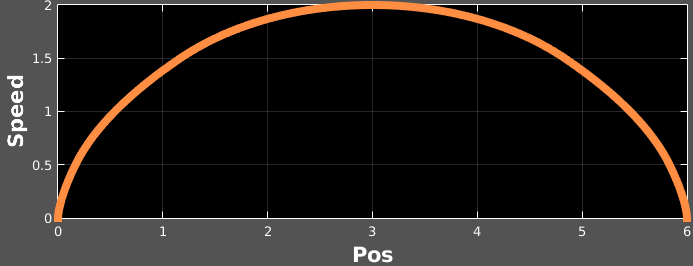
\includegraphics[width=0.4\columnwidth]{graphics/6phase_v(s).png}
  \label{fig:6phaseprofile}
  } &
  \subfigure[4 phase profile] {
  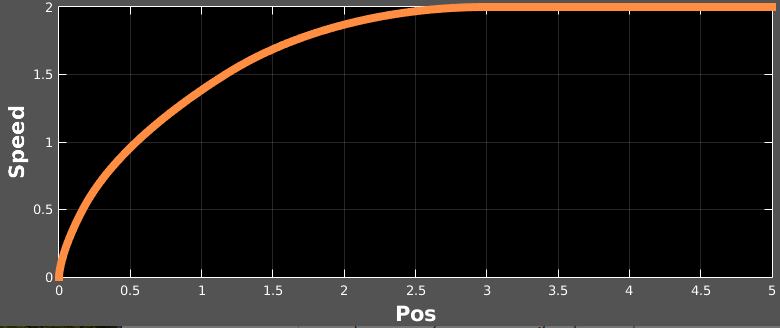
\includegraphics[width=0.4\columnwidth]{graphics/4phase_v(s).png}
  \label{fig:4phaseprofile}
  } \\
  \subfigure[4 Reversed phase profile] {
  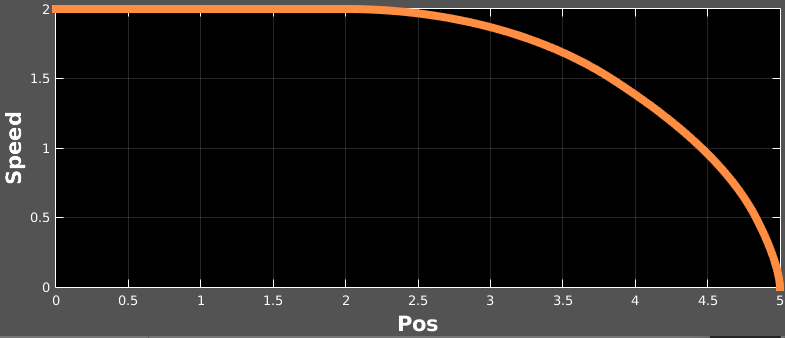
\includegraphics[width=0.4\columnwidth]{graphics/4Rphase_all_derivatives.png}
  \label{fig:4rphaseprofile}
  } &
  \subfigure[3 phase profile] {
  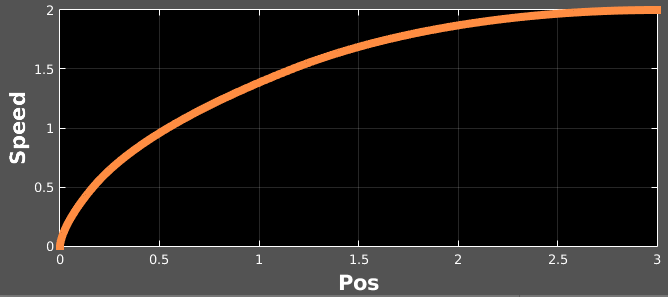
\includegraphics[width=0.4\columnwidth]{graphics/3phase_v(s).png}
  \label{fig:3phaseprofile}
  }
  \end{tabular}
  \caption{6, 4, 4Reversed and 3 phase profiles, displayed as speed vs. position along path}

\end{figure}

\subsubsection{4 Phase} \label{sec:4phase}

When $v_i < v_m \simeq v_f$, the vehicle should increase speed, then maintain that speed for the distance remaining in the segment.


\subsubsection{Reversed 4 Phase} \label{sec:reversed4phase}

When $v_i \simeq v_m > v_f$, it would be nonsensical to immediately brake.
The initial speed is maintained for a period before applying the brakes.


\subsubsection{3 Phase} \label{sec:3phase}

A change from one speed to another.
All of the above profiles are composed of some combination of a 3 phase profile and a $j_k = 0$ phase.
This presents a difficulty in that either $L$ or $v_f$ may be enforced, but not both (there is no solution to enforce both).
As such, this profile is chosen only for a segment in which it is impossible to completely arrive at the end speed given the initial speed, so fitting one of the two 4 phase profiles has been attempted and subsequently failed.

%%%%%%%%%%%%%%%%%%%%%%%%%%%%%%%%%%%%%%%%%%%%%%%%%%%%%%%%%%%%%%%%%%%%%%%%%%%%%%%%

\subsection{Path Segmentation} \label{sec:pathsegmentation}

% make sure to incorporate extensibility to other constraints
The goal of the segmentation process is to divide a given path into multiple portions where each has a uniform upper limit on speed, acceleration, and braking.
There are 3 steps in the segmentation process:
\begin{enumerate} \label{asdf}
  \item \emph{Ceiling calculation}, where $\mathbf{b}$, $\mathbf{a}_m$, and $\mathbf{j}_m$ are found for every point in the given path.
  \item \emph{Clustering}, in which path points are grouped sequentially.
  \item \emph{Consolidation}, in which a single $\mathbf{b}$, $\mathbf{a}_m$, and $\mathbf{j}_m$ is selected for each segment.
\end{enumerate}
After this is done, the process described in Section \ref{sec:jerkprofiles} may be applied to each of the segments.

The ceiling calculation is a minimax problem.
Each of the 9 scalars is a minimum of several maxima computed from an arbitrary set of constraints.
For instance, acceleration constraints may include a set of limits derived from friction coefficients at every point along the path.

% How we actually did this.
For the purposes of developing a simple example application, two constraints will be used for $v_{m,k}$: legal speed limit ($SL$, set constant for the whole path) and lateral acceleration limit $a_{B,y}^{max}$. 
Lateral acceleration constraints are translated into longitudinal speed constraints using the approximation $v_{m,k}(a_{B,y}) = \sqrt{a_{B,y}^{max}/\kappa_k}$ for $k = 1, ..., N_p$, where $N_p$ is the number of waypoints in the full path.
\emph{RG: this is the first place we introduce two subscripts. please explain what the two subscripts stand for in general for example in $a_{B,y}$ and $v_{m,k}$ ?????? }
The value $\kappa_k$ denotes the path curvature at each point.
For each path point, the value $v_{m,k}(a_{B,y}^{max})$ denotes the speed necessary to obtain the limit lateral acceleration, denoted by $a^{max}_{B,y}$.

This information is used to choose the segment boundaries in the clustering step.
Any number of clustering algorithms may be used here, and prudent choice of segment boundaries is arguably one of the most critical pieces of trajectory planning process.
For the present example, we will choose a simple univariate heuristic which essentially identifies curves in the roadway.
Each time that $v_{m,k} < SL$ becomes true, a curve is beginning, and a segment boundary is drawn.
Each time that $v_{m,k} = SL$ is once again true, the current curve has ended, and another segment boundary is drawn.
Figure \ref{fig:1Dto2DandSegmentation} shows the result of this algorithm. 

% \begin{figure}[thpb]
%   \centering
%   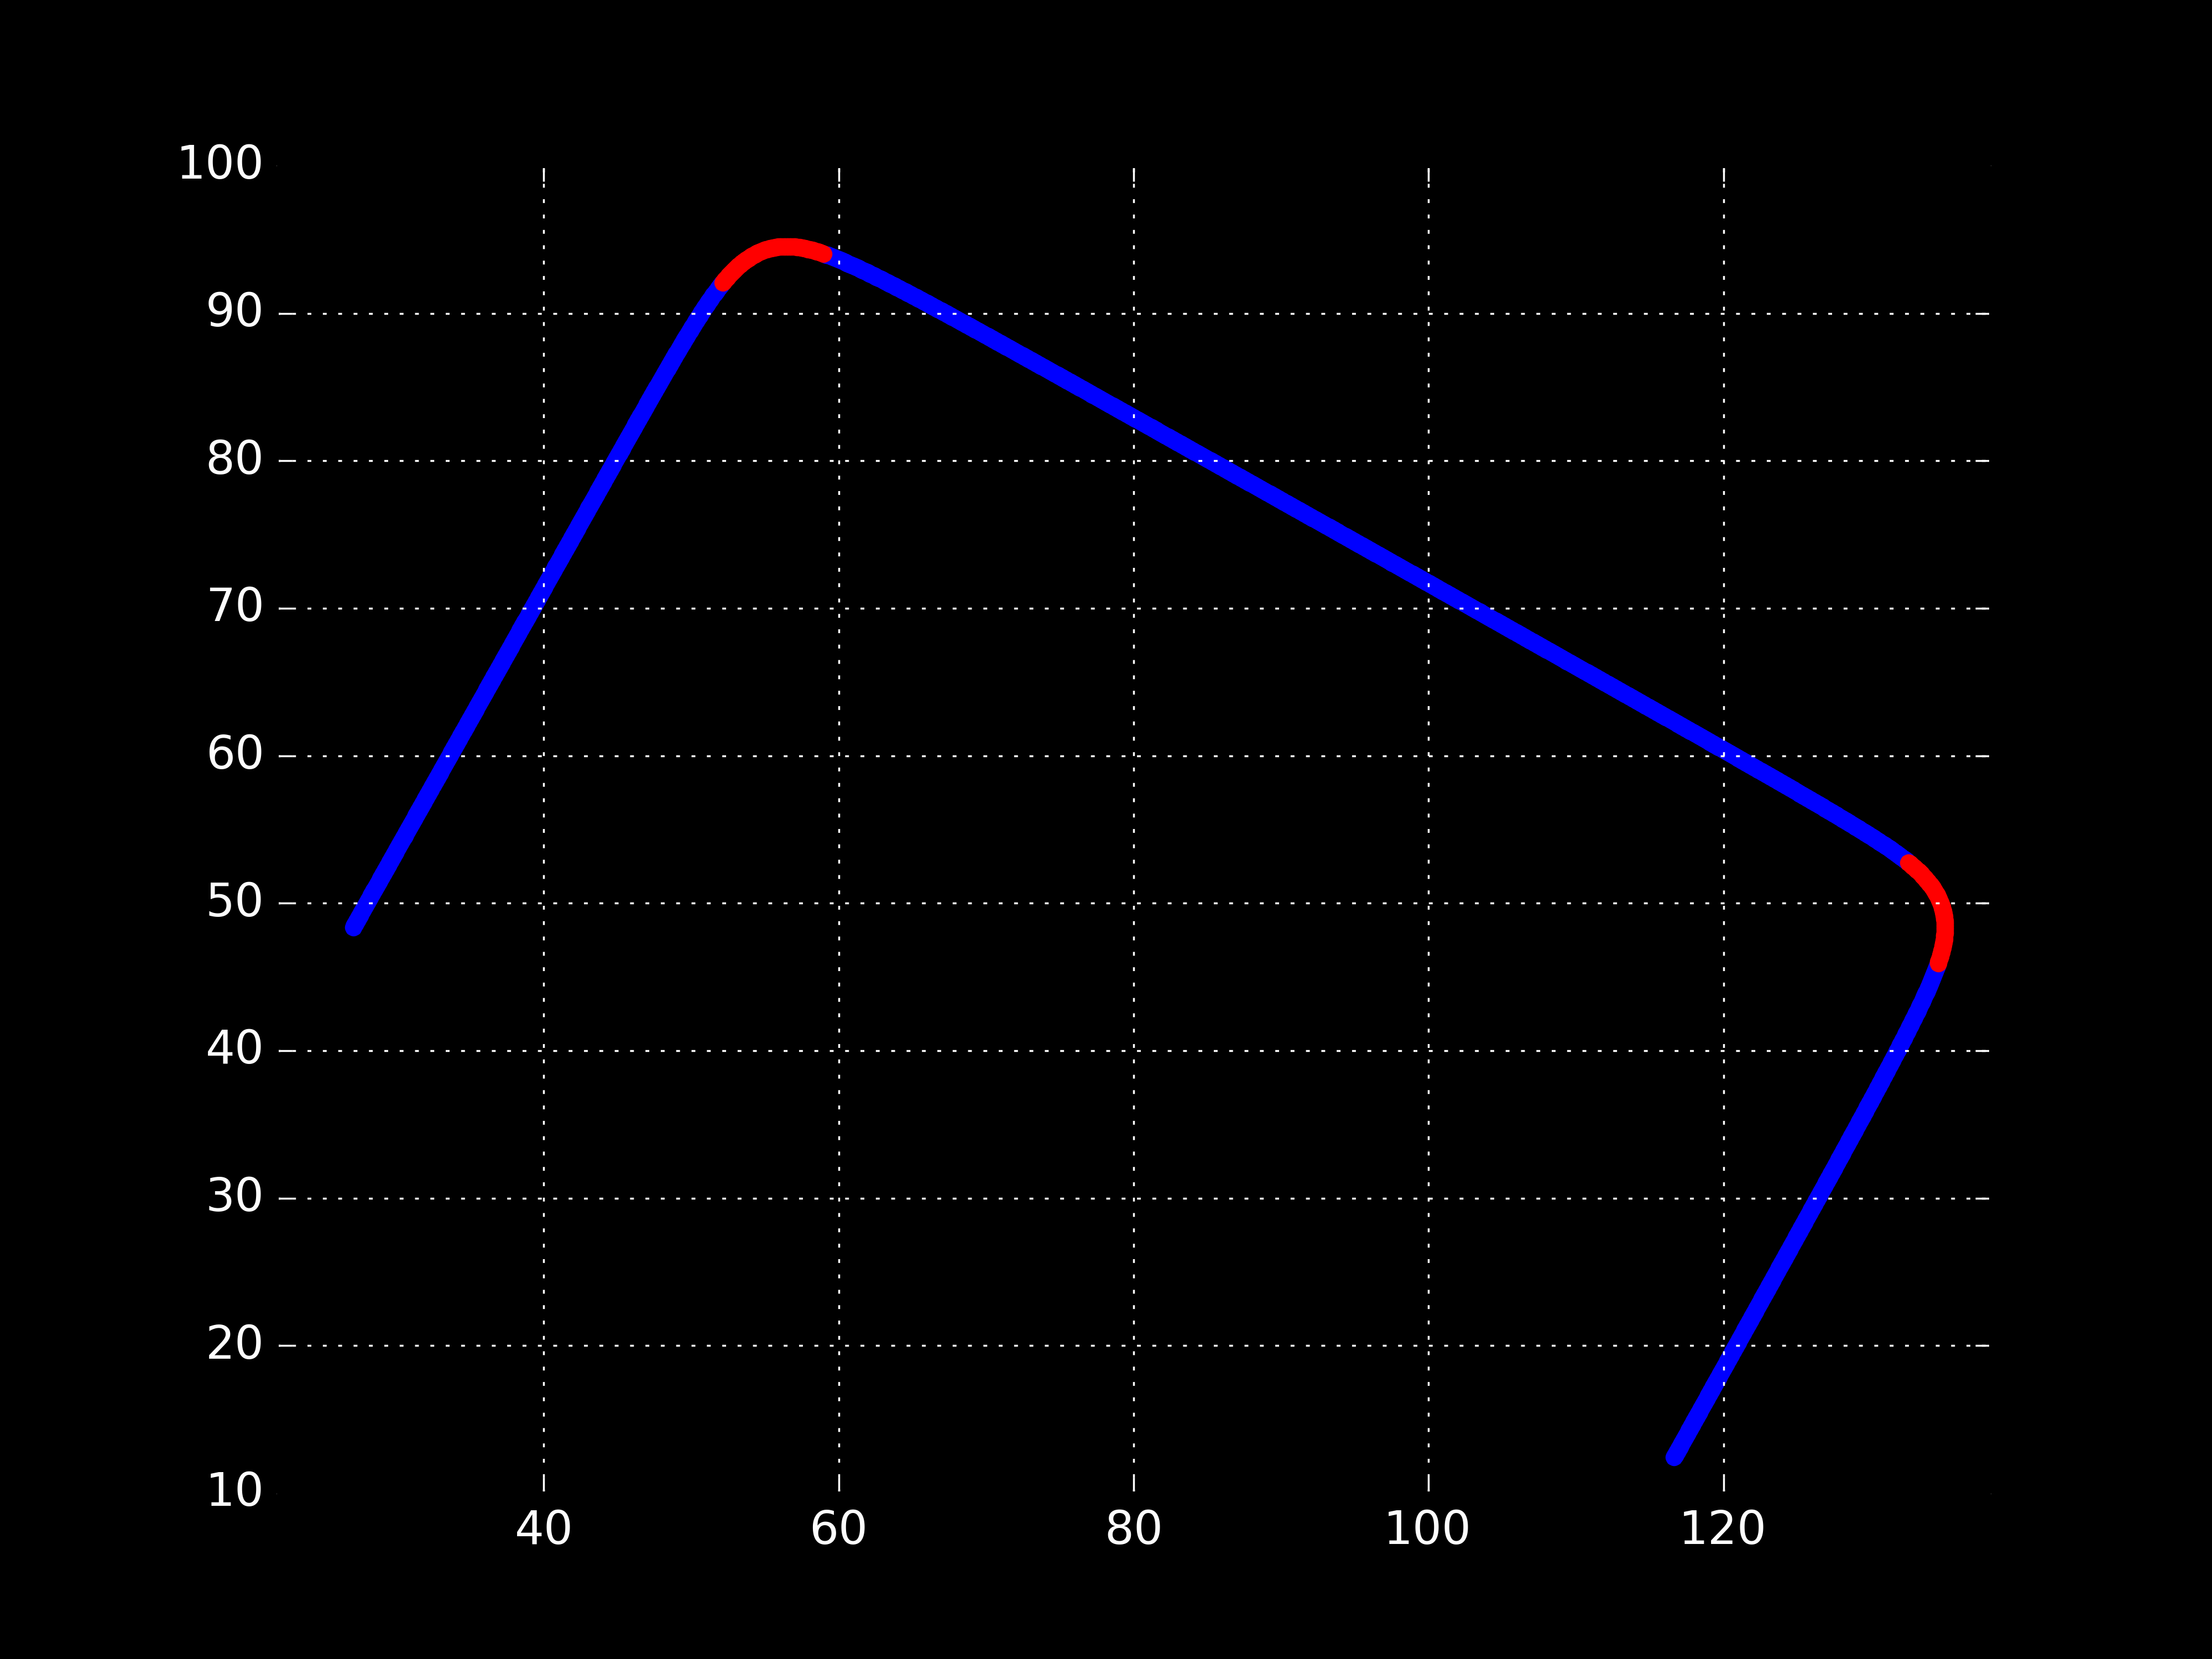
\includegraphics[width=0.8\columnwidth]{graphics/course_highlighted_turns.png}
%   \caption{
%     Clustering output for a short path when using an algorithm which draws segment boundaries around curves.
%     Portions in red indicate areas where the longitudinal speed required to adhere to lateral acceleration limits is below the legal speed limit of 11.176 m/s (25 mi/hr).
%   }
%   \label{fig:course_highlight_turns}
% \end{figure}

% \begin{figure}[thpb]
%   \centering
%   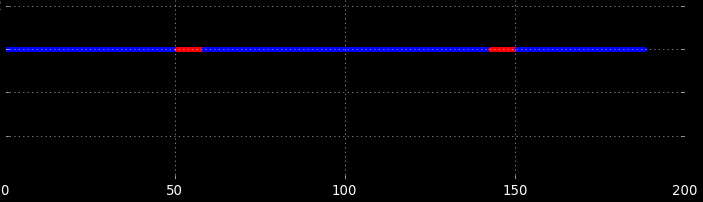
\includegraphics[width=1.0\columnwidth]{graphics/1Dsegmentation.png}
%   \caption{Showing the path projected onto the one dimensional s coordinate system}
%   \label{fig:scoord}
% \end{figure}

% \begin{figure}[thpb]
%   \centering
%   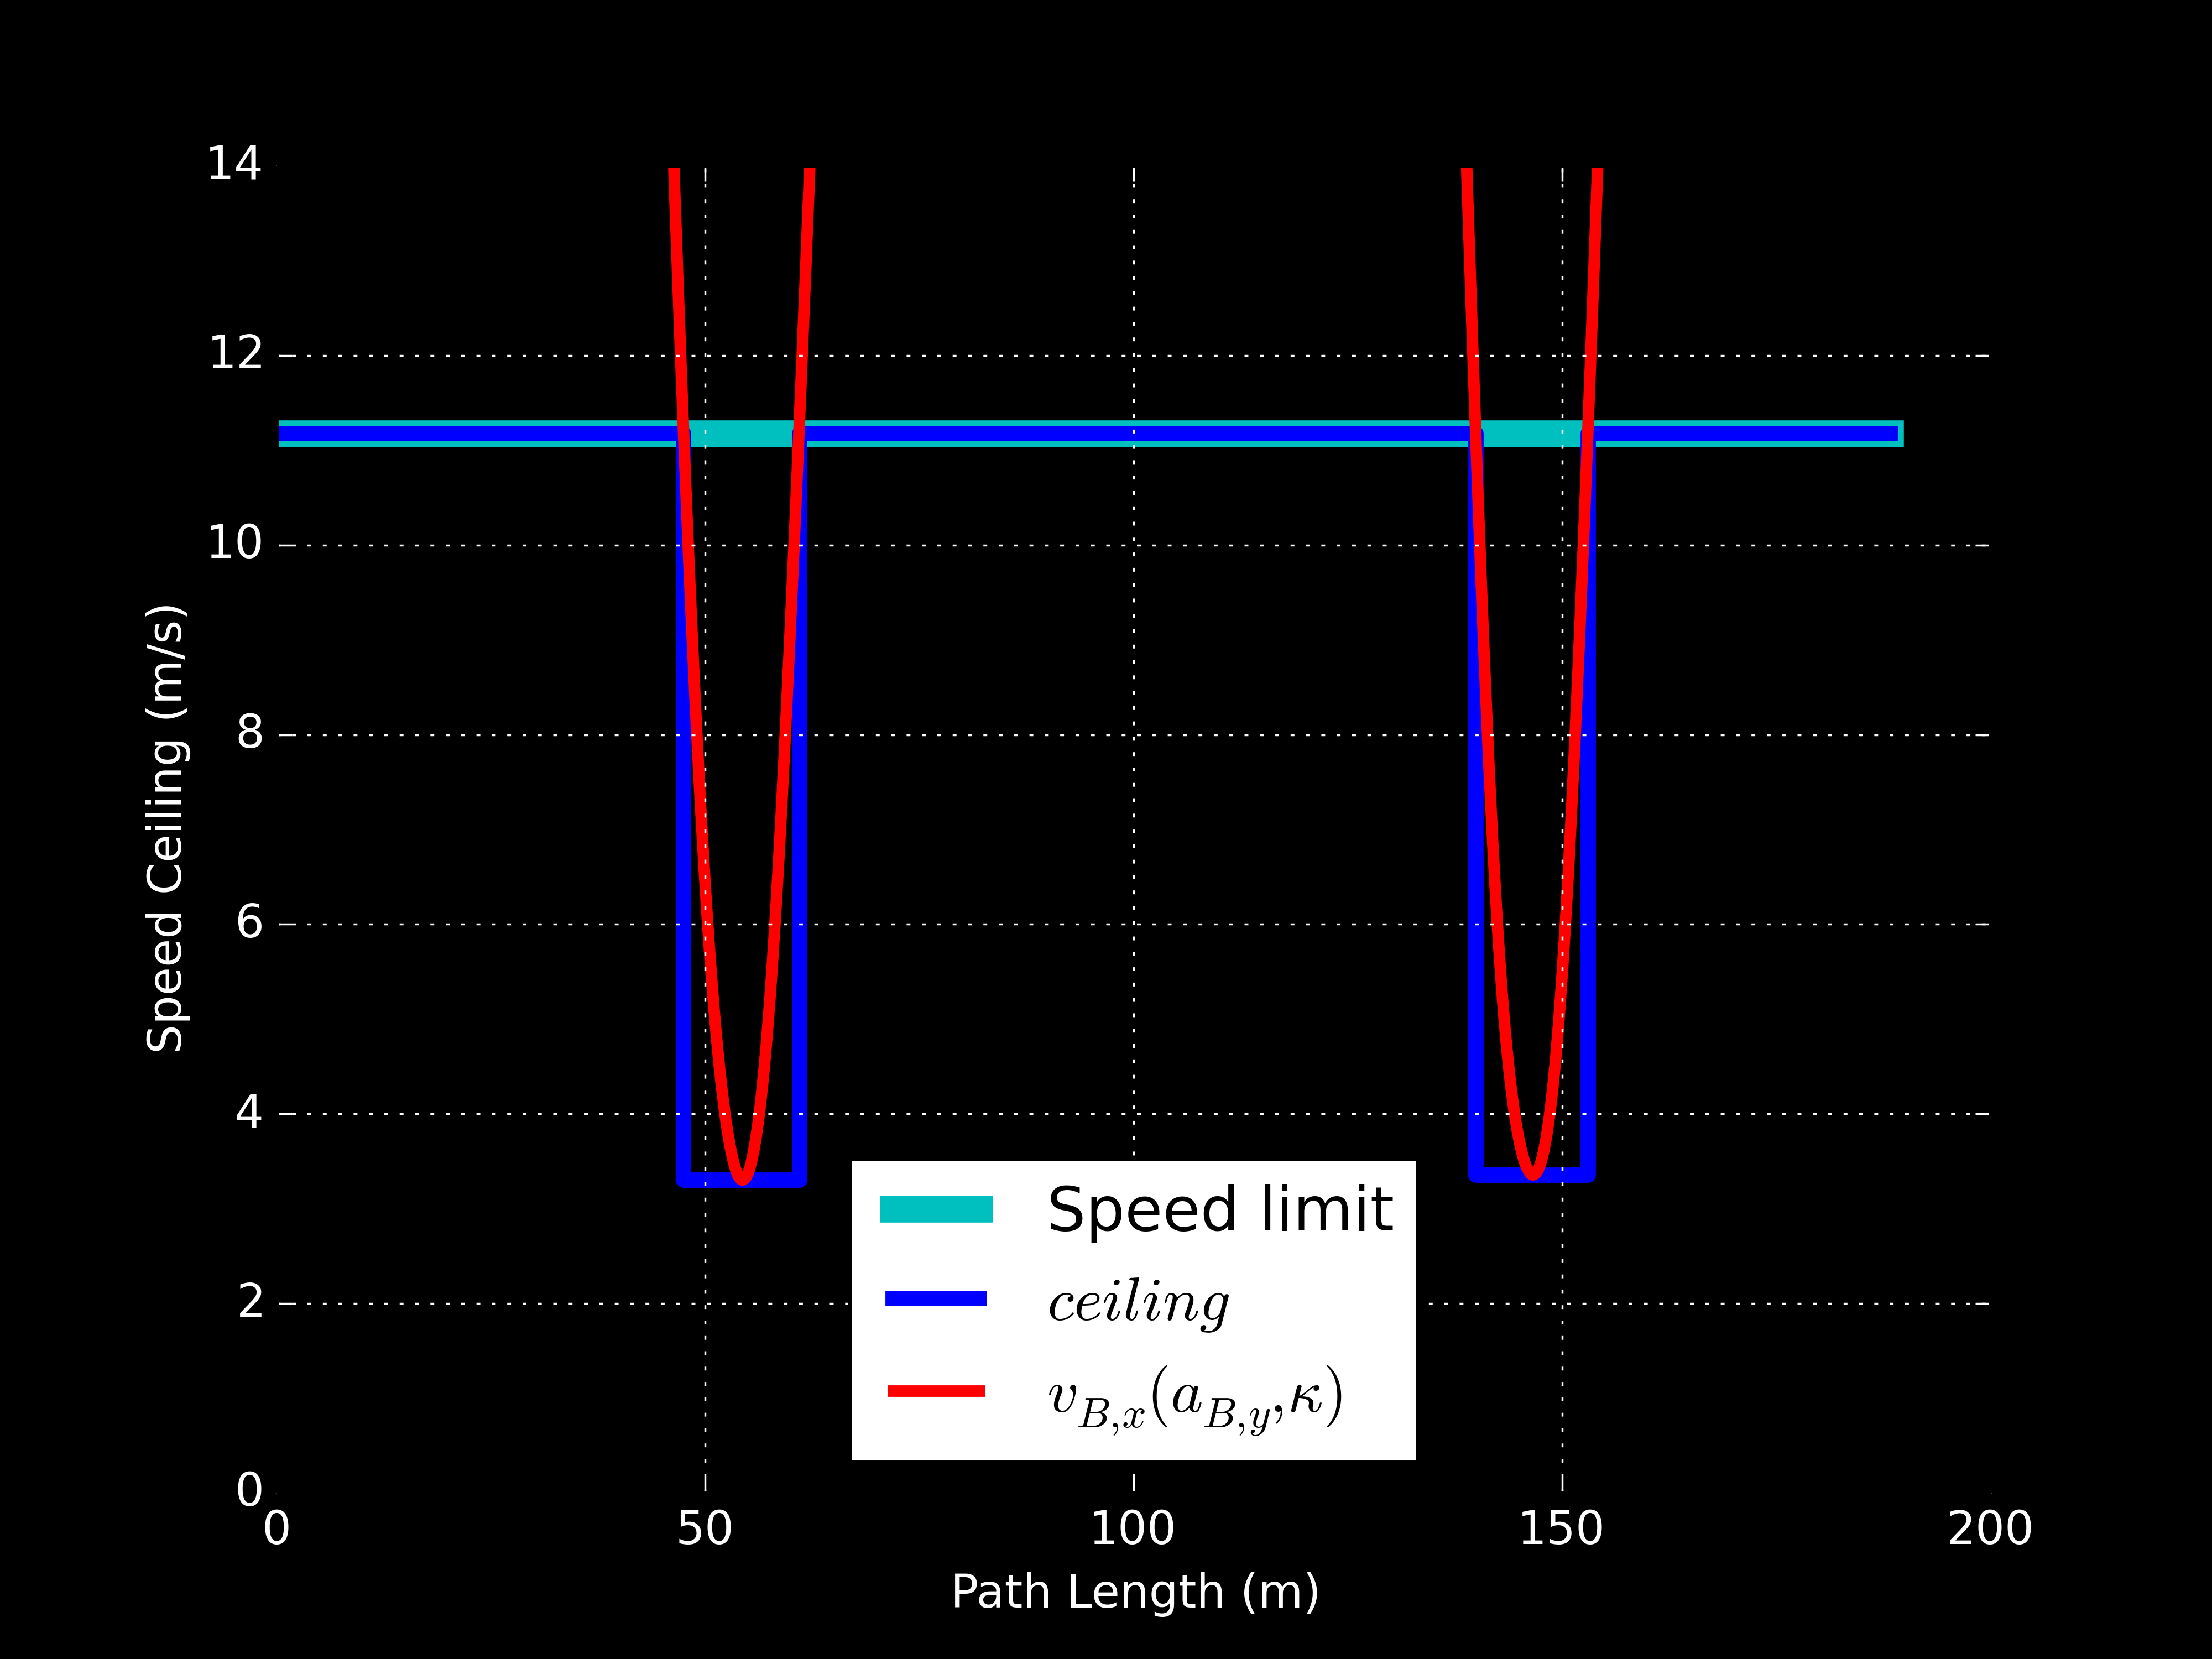
\includegraphics[width=0.8\columnwidth]{graphics/speed_ceiling.png}
%   \caption{
%     Example of $v_m$ consolidation for simple univariate path clustering which corresponds the the path shown in Figure \ref{fig:course_highlight_turns}.
%     The legal speed limit of 11.176 m/s (25 mi/hr) is shown in cyan.
%     The longitudinal speed required to adhere to lateral acceleration limits is shown in red.
%     The resultant speed ceiling is shown in blue.
%   }
%   \label{fig:consolidation_speed_ceiling}
% \end{figure}

\begin{figure}[thpb]
  \centering
  \subfigure[
    Clustering output for a short path when using an algorithm which draws segment boundaries around curves.
    Portions in red indicate areas where the longitudinal speed required to adhere to lateral acceleration limits is below the legal speed limit of 11.176 m/s (25 mi/hr).
  ]{
    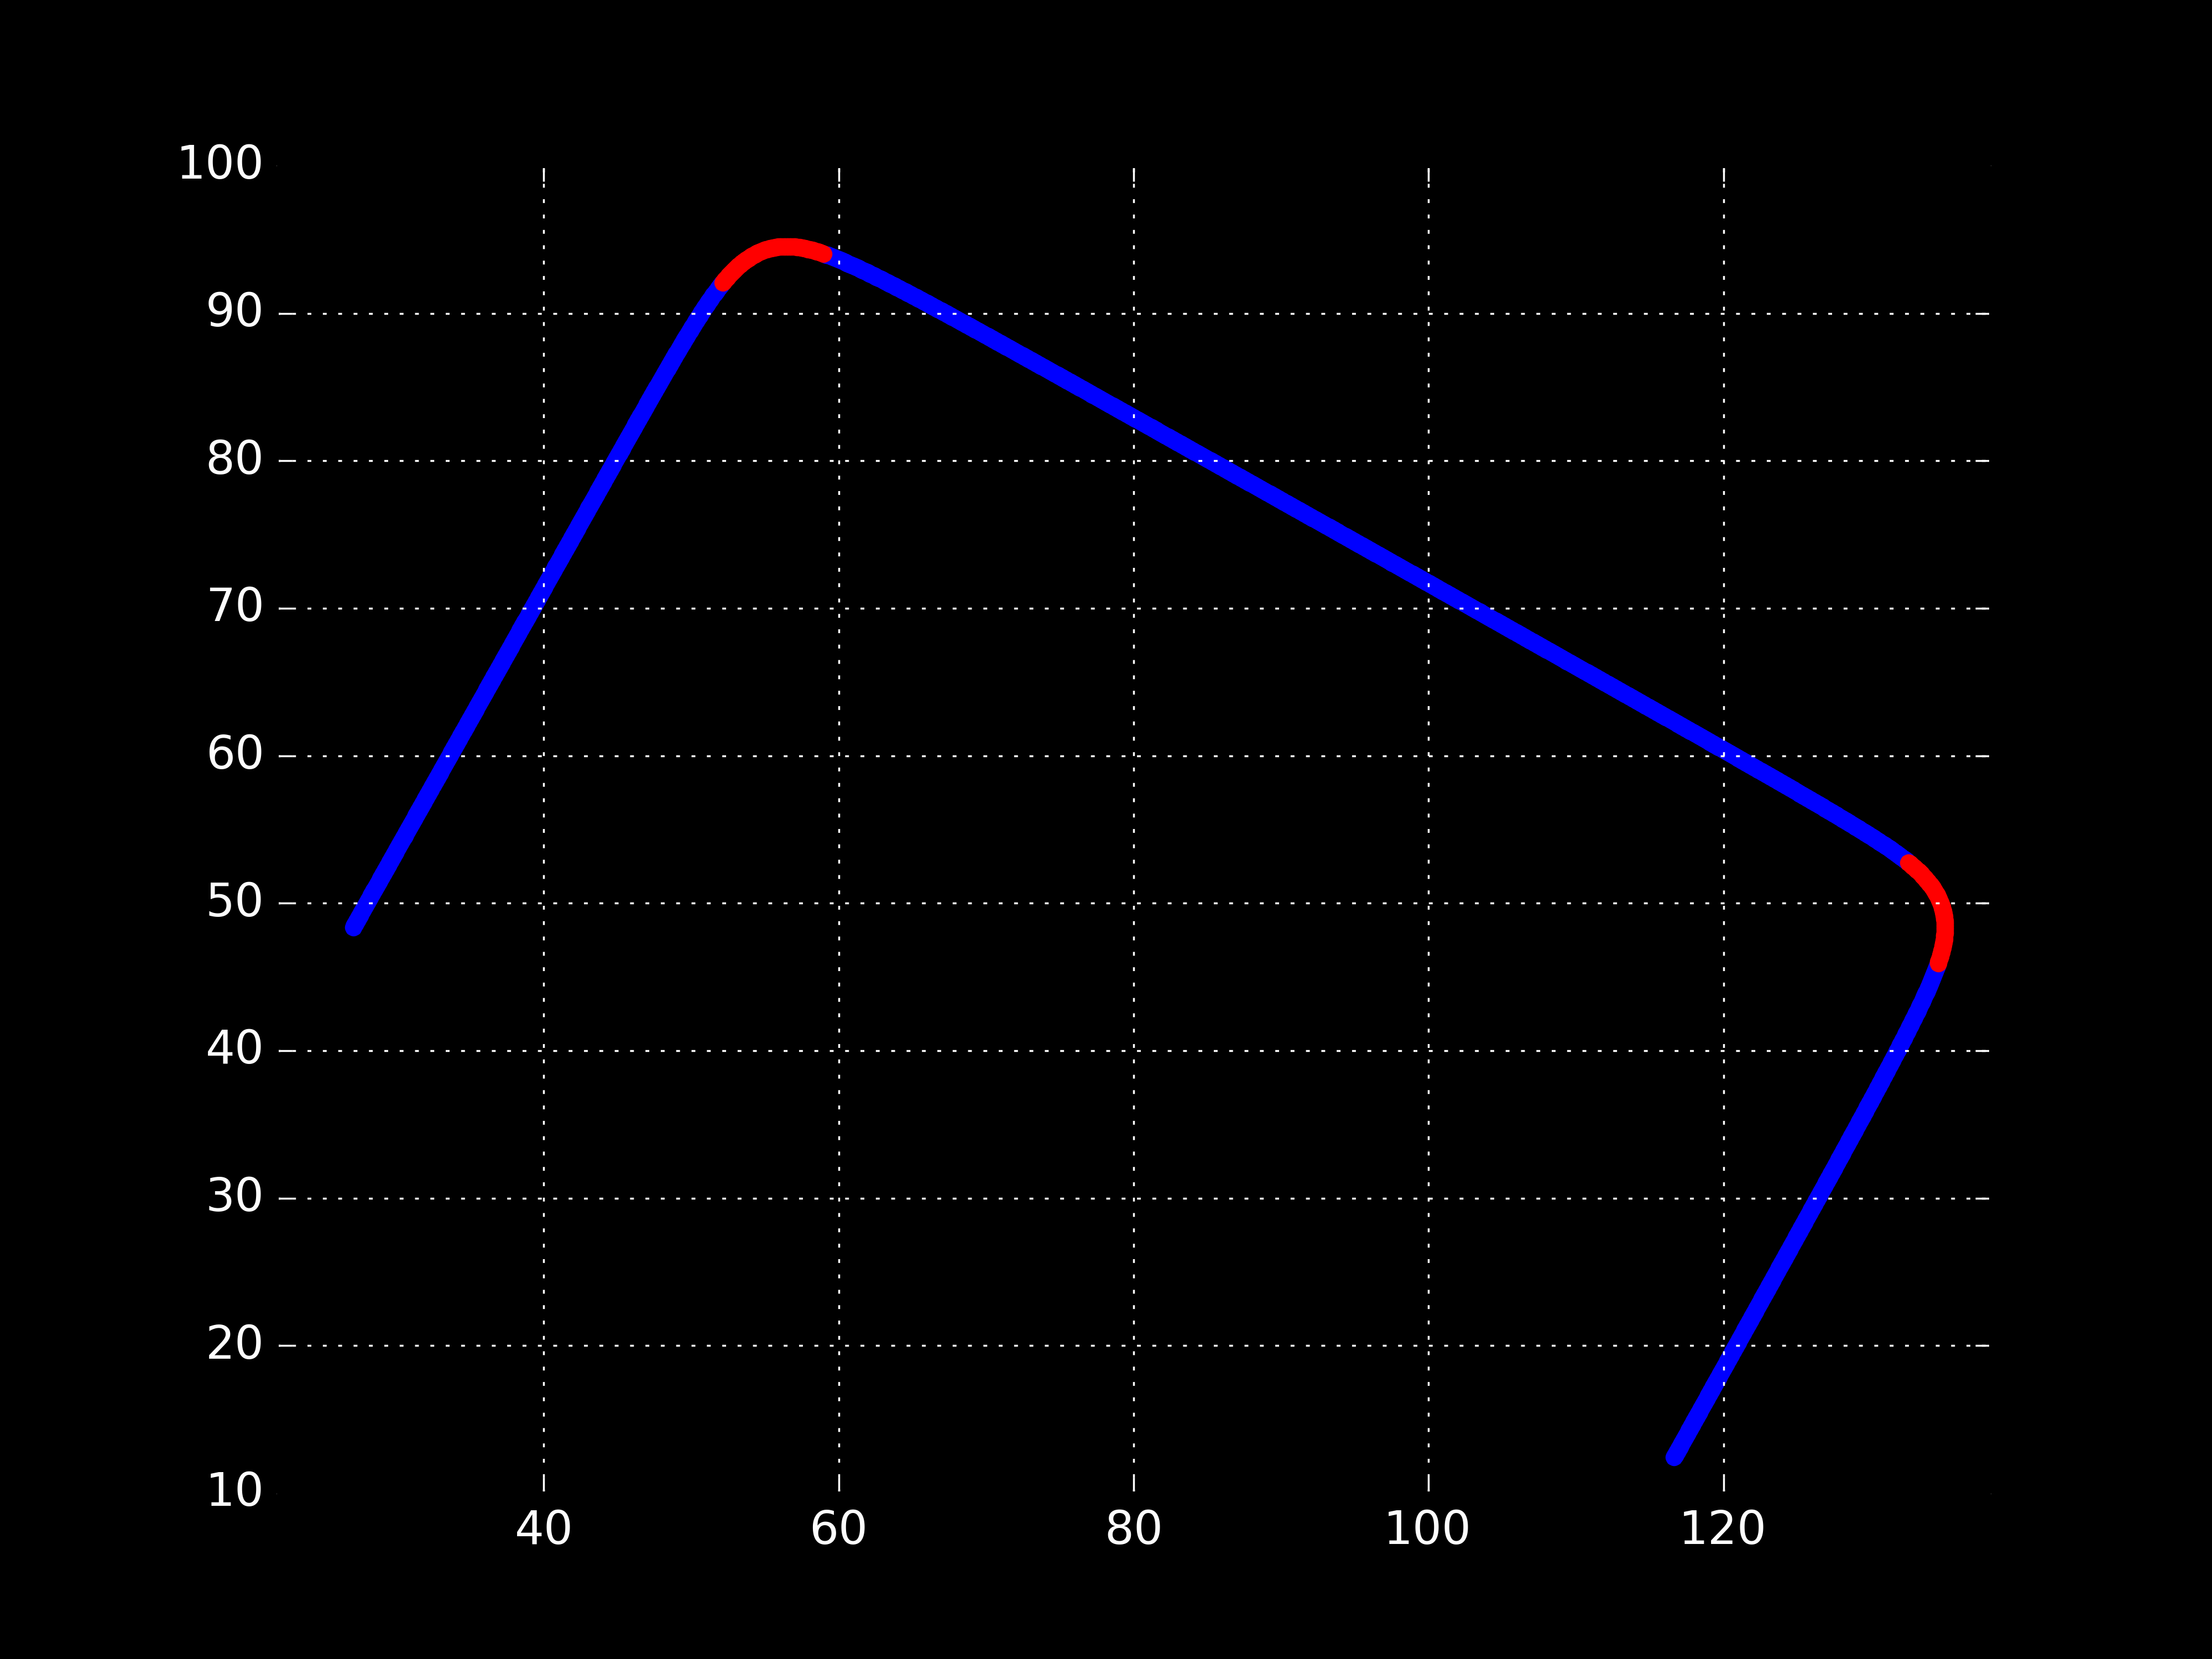
\includegraphics[width=0.8\columnwidth]{graphics/course_highlighted_turns.png}
  }
  \\
  % \subfigure[
  %   Showing the path projected onto the one dimensional s coordinate system
  % ]{
  %   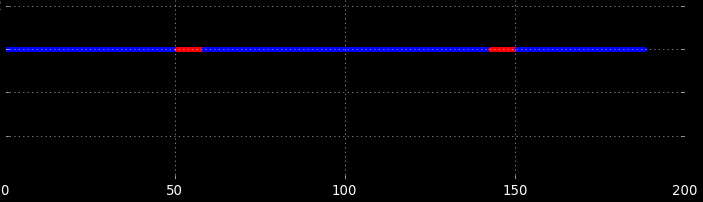
\includegraphics[width=1.0\columnwidth]{graphics/1Dsegmentation.png}
  % }
  % \\
  \subfigure[
    Example of $v_m$ consolidation for simple univariate path clustering which corresponds to the path shown above.
    The legal speed limit of 11.176 m/s (25 mi/hr) is shown in cyan.
    The longitudinal speed required to adhere to lateral acceleration limits is shown in red.
    The resultant speed ceiling is shown in blue.
  ]{
  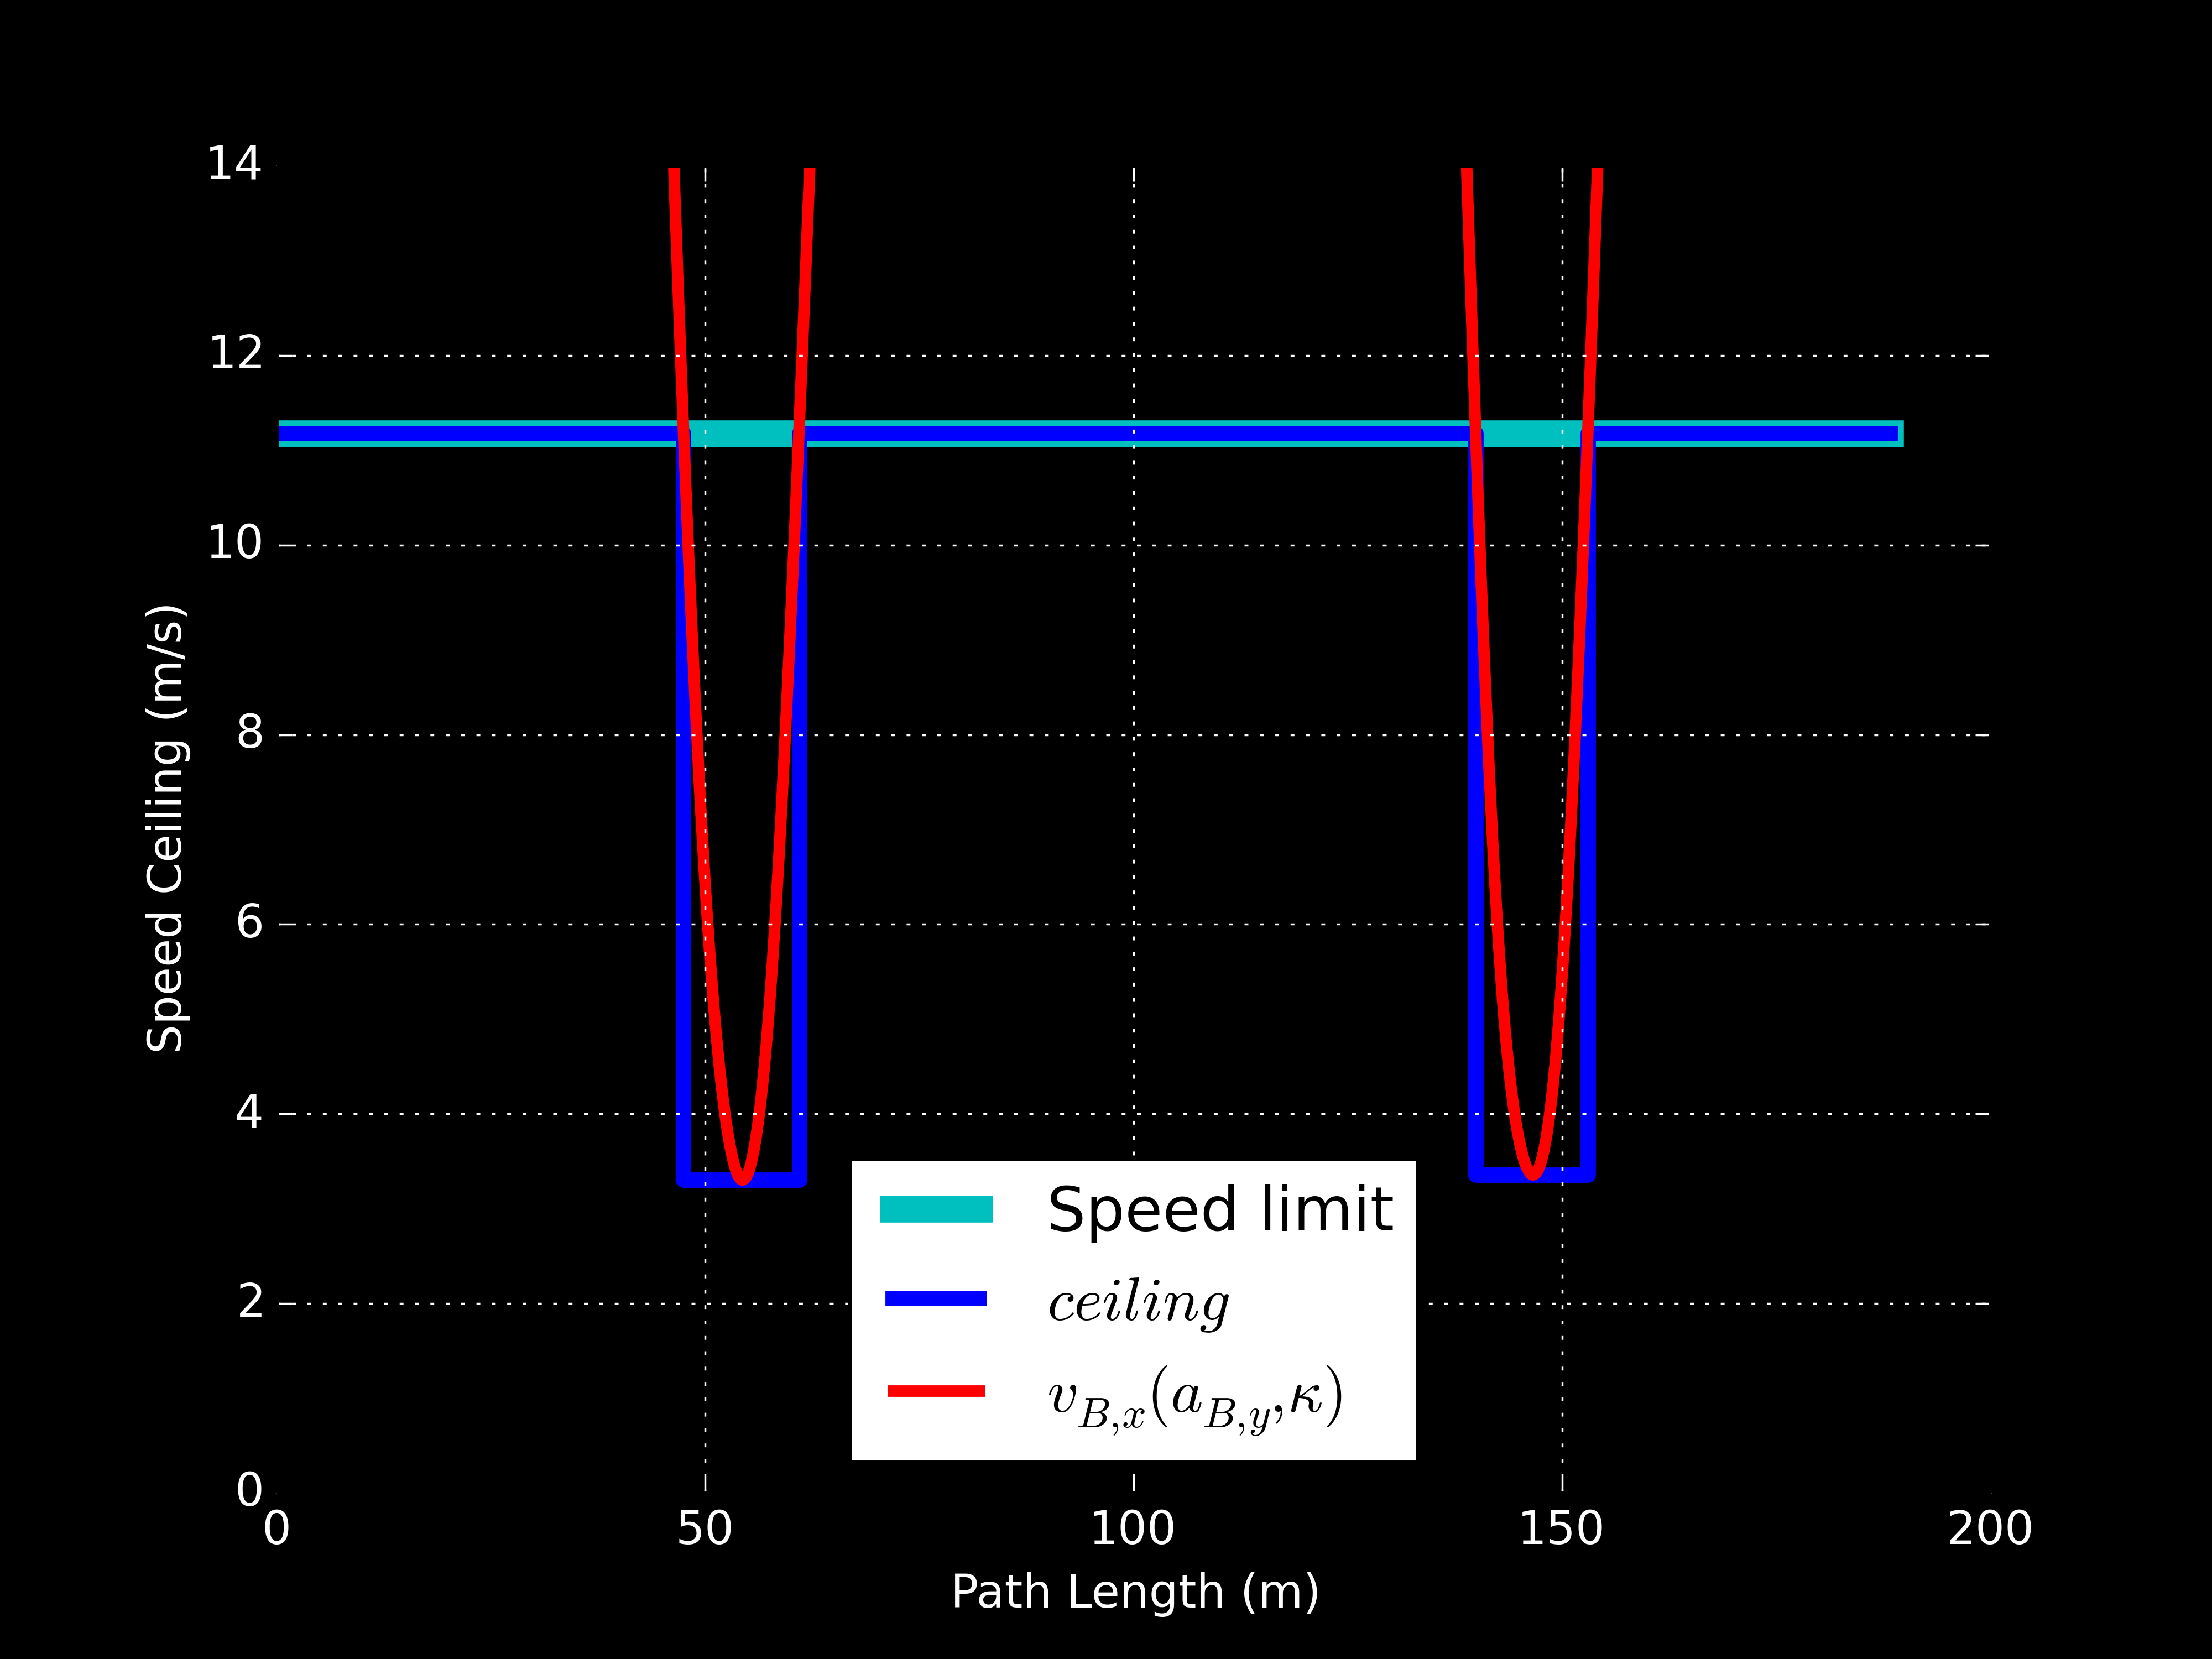
\includegraphics[width=0.8\columnwidth]{graphics/speed_ceiling.png}
  }
  \caption{Path segmentation and speed ceiling consolidation procedures.}
  \label{fig:1Dto2DandSegmentation}
\end{figure}

% need better notation here.
In the consolidation step, a single set of $\mathbf{g}$, $\mathbf{a}_m$, and $\mathbf{j}_m$ must be calculated for each segment using the values corresponding to each of the path points which comprise the segment in question.
The minimum of scalar across all constituent points is chosen.
While not time optimal, it does ensure that no constraints are violated while still keeping the number of total segments low.
In the present example, this means that in the straight portions of the path $v_m = SL$ and in the curves $v_m$ is set to the value required to obtain $a_{B,y}^{max}$ for the entirety of the curve.
As a result, many of the curves will have a constant speed.
For the sake of simplicity, the values of $a^+_{m,k}$, $a^-_{m,k}$, $j^+_{m,k}$, and $j^-_{m,k}$ are all set constant for the entire path, using values from \cite{Maurya2012,Hoberock1977,Long2000}.

%%%%%%%%%%%%%%%%%%%%%%%%%%%%%%%%%%%%%%%%%%%%%%%%%%%%%%%%%%%%%%%%%%%%%%%%%%%%%%%%

\subsection{Unified Solution} \label{sec:unifiedsolution}

At this point, the path has been divided into segments and conditions have been computed such that an analytically derived plan can be fit to each segment individually.
Now a reference trajectory must be generated for the entire path.
Continuity of position, speed, and acceleration is the primary goal of this process.

A jerk vs. time profile is fit to each segment using the algorithm in Section \ref{sec:jerkprofiles}.
Speed and acceleration must be continuous between each segment, but only the corresponding speed ceilings have been found, so the start and end conditions for each segment must be determined.
The values of $a_i$ and $v_i$ for the first segment is set to be the value which is currently reported from sensor data.
Since the final acceleration is set to zero for all profiles, each subsequent segment may begin with $a_i = 0$.
For the final segment, setting $v_f = 0$ is prudent unless the scenario demands otherwise.
Algorithm~\ref{alg:segmentspeedboundaryconditions} is used to set boundary speed conditions for the interior segments. 

\begin{figure}
  \begin{algorithmic}[1]
    \Procedure{SegmentBoundarySpeeds}{$v_m$}
      \State $\mathbf{v}_p \gets \mathbf{v}_m$ \Comment{Initialize targets as ceilings}
      \State $\mathbf{v}_{p,0} \gets v_i$ \Comment{Set starting speed to current}
      \State $\mathbf{v}_p = [\mathbf{v}_p, 0]$ \Comment{Add final speed of 0}
      \For{$i = 1, ..., N_s-1$}
        \If{$v_{m,i+1} > v_{m,i}$}
          \State $v_{p,i+1} \gets v_{m,i+1}$
        \Else
          \State $v_{p,i+1} \gets v_{m,i}$
        \EndIf
      \EndFor
    \EndProcedure
  \end{algorithmic}
  \caption{
    Algorithm to set speed boundary conditions for interior path segments.
    Having consolidated the waypoints in to a set of path segments, the maximum allowable speed for each segment, $v_{m,i}$ is known.
    This algorithm uses the set of $\mathbf{v_{m}}$ for all segments to choose the highest allowable start and end speeds for each path segment.
  }
\label{alg:segmentspeedboundaryconditions}
\end{figure}

% talk about control points
Now each segment is solved individually.
In the case where a segment requires a speed change which is infeasible given limits on acceleration and jerk, then the final speed for that segment is planned to be the closes possible value.
When these discrepancies in the feasible $v_f$ for a segment arise, the corresponding value in $v_p$ is updated so that the new conditions may be accounted for in the subsequent segment.

At the end of the process, there will be a set of $N_{cp}$ ``control points''.
A control point is a vector $[t_{ref}, s, v_{B,x}, a_{B,x}, j_{B,x}]$ which describes the longitudinal kinematic state of the target vehicle at the moment of an infinite jounce jerk change.
Fitting a jerk profile to each segment results in control points which must be stitched into the control points for the preceding segments.
While no further information than initial conditions, time durations, and jerk values is needed (simple integration would yield lower derivatives of position), this information is already available since it must be solved for each segment.
This extra information may be used as a redundancy layer to verify that no errors occurred.
For each segment with $M$ jerk phases, the following is produced:
\begin{itemize}
  \item $M$ time durations $\Delta t_{ref}$. These must be added to the last time value from the previous segment to translate them into reference time.
  \item $M+1$ values of distance elapsed within the segment $\Delta s$. These must be shifted forward by the last $s$ value from the previous segment to translate them into the 1D path domain. Additionally, the first value must be erased.
  \item $M+1$ values of $v_{B,x}$. The first value is checked against the last value from the previous segment to verify equality, then it is erased. These need no translation.
  \item $M+1$ values of $a_{B,x}$. The first value is checked against the last value from the previous segment to verify equality, then it is erased. These need no translation.
  \item $M$ jerk values, which may be appended directly to the preceding jerk values
\end{itemize}

\emph{RG: please explain reference time, $s$ and $\Delta s$ ????????}

After stitching together control point vectors for time, position, and its derivatives, all information required to have a trajectory plan is now in place.
Since $j(t)$ is piecewise constant, it may be integrated to determine an instantaneous trajectory at any moment in time.
To aid in this, univariate splines are created with time as the independent variable, using the control points as knots.
Position along the path as a function of reference plan time, $s(t)$, takes the form of a cubic Hermite spline, constructed using the speed control points $v_{B,x}(t)$ to set the derivatives.
Speed along the path $v_{B,x}(t)$ takes the form of a quadratic Hermite spline, with the acceleration control points $a_{B,x}(t)$ used to set the derivatives at every knot.
Acceleration $a_{B,x}(t)$ is piecewise linear, so lookup is a trivial matter.
The same applies to $j_{B,x}(t)$, which may be implemented with a simple table.

However, the time at which the trajectory plan must be referenced is not always known.
The solution to this problem is known as trajectory tracking control, and will be discussed in the next section.

%%%%%%%%%%%%%%%%%%%%%%%%%%%%%%%%%%%%%%%%%%%%%%%%%%%%%%%%%%%%%%%%%%%%%%%%%%%%%%%%

\subsection{Reactive Stop Trajectories} \label{sec:reactivestoptrajectory}

This is the procedure for determining nominal stopping distance required.
A 3 phase profile will be used, with end conditions $v_f=0, a_f=0$ and initial conditions set to the current state of the navigation filter.

While it would seem that the segment solving procedure described in Sec. \ref{sec:3phase} could be applied to reactive stopping, this is not the case.
As was mentioned previously, only one of $[L, v_f]$ may be rigidly enforced for a 3 phase profile, but not both, since no closed-form solution exists for that case.
Normal planning enforces $L$ to avoid skewing segment boundaries within each subpath.
However, reactive stopping requires that $v_f$ be enforced, and that we solve for $L$.
Reformulating a new 3 phase jerk profile accordingly is a simple matter for a symbolic solver.
%%% This is the brief way of wording the preceding three sentences.
% The trajectory planner uses total distance as parameter, and is not suitable for our purpose as the end speed constraints are not met. So we reformulate and replace $L$ with $v_f$ as the hard constraint.

Now appropriate values of $a_m^-$ and $j_m^-$ must be chosen to completely parameterize the trajectory.
For calculating $\Delta s_{RSTOP}$, the same set of values from normal planning is used.

Once the path manager triggers RSTOP, the trajectory is then recomputed with increasingly higher-magnitude values of $a_m^-$ and $j_m^-$ until $\Delta s_{RSTOP} <= \Delta s_{avail}$.
Should one of the values $a_m^-$ or $j_m^-$ required to fulfill this condition exceed the limits $a_m^{-,max}$ or $j_m^{-,max}$, then limit braking parameters are set such that $a_m^-=a_m^{-,max}$ and $j_m^-=j_m^{-,max}$, and the user is alerted.

After this, the spline creation procedure detailed in Sec. \ref{sec:unifiedsolution} is performed.
The path must now be truncated for 1D $\leftrightarrow$ 2D transformation.
Within the trajectory tracker, all portions of the path leading up to the location of RSTOP triggering are removed, as well as the portions after the location which corresponds to $s_{veh} + \Delta s_{RSTOP}$
This is depicted in Fig. \ref{fig:pathtostop}
The vehicle now begins sampling from this trajectory and is executing a smooth reactive stop.

\begin{figure}[thpb]
  \centering
  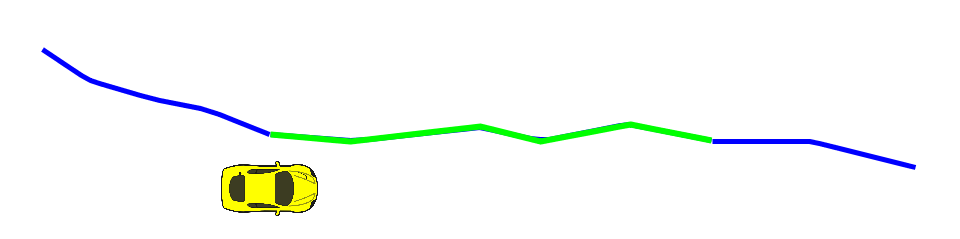
\includegraphics[width=1.0\columnwidth]{graphics/RSTOP_path_truncation.png}
  \caption{Green color path is the one over which the car finds a trajectory to stop. please show green as dashes for b\&w printing ??????????? }
  \label{fig:pathtostop}
\end{figure}


%%%%%%%%%%%%%%%%%%%%%%%%%%%%%%%%%%%%%%%%%%%%%%%%%%%%%%%%%%%%%%%%%%%%%%%%%%%%%%%%
%%%%%%%%%%%%%%%%%%%%%%%%%%%%%%%%%%%%%%%%%%%%%%%%%%%%%%%%%%%%%%%%%%%%%%%%%%%%%%%%

\section{Trajectory Tracking} \label{sec:trajectorytracking}

After planning has been performed, a reference signal must be regularly supplied to a control system in order for the vehicle to carry out the plan.
This is known as tracking control.
The primary difficulty here is that the trajectory plan has been developed in a one dimensional position space using a reference time which will have unknown drift relative to real time.
As such, we must find a way to look up the coordinates of the vehicle within the reference trajectory using information typically available for autonomous cars.
A minimal set of such information would include position, velocity vector, heading, and acceleration in the body frame.
After this, it is assumed that the vehicle controller will need samples of a small window into the future trajectory to pilot the vehicle.

\begin{figure}[thpb]
  \centering
  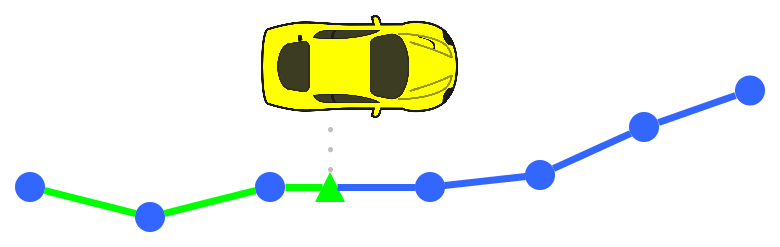
\includegraphics[width=0.5\columnwidth]{graphics/PathProjection.png}
  \caption{Showing projection of current position of car shown by green triangle to s coordinate system}
  \label{fig:cartos}
\end{figure}

The general idea is to project the vehicle's current position onto the path then find the cumulative distance along the path between the start point and the projection point.
This is the 1D location corresponding to the vehicle's current reference time.
Once this reference time is obtained, it may be used to look up position, speed, acceleration, and jerk along the curve of the path over the future time window.
From there it is a matter of simple geometry to transform these values into the coordinate system of the path and, subsequently, any other coordinate system which may be needed.

% \subsection{Path Projection} \label{sec:pathprojection}

Several algorithms exist to find the optimal projection of the target vehicle's present kinematic state (position, velocity, and acceleration vectors) onto the path.
A simple approximation is to perpendicularly project the vehicle's position onto a series of lines running between each pair of adjacent points in the path (this will be referred to as a ``link'', and is depicted in Fig. \ref{fig:cartos}).
Projections which lie outside of the link's two constituent path points are snapped to that which is nearest.
The projection which is closest to the vehicle's actual position is then assumed to be the correct path projection $\mathbf{r}_p$.
Any number of modifications can be made using heading, velocity vectors, and previous information to allow this method to be extended to complex paths which overlap or self-intersections.

Choosing an algorithm to obtain the current one dimensional position of the vehicle along the length of the path $s_{veh}$ (i.e., in the same one-dimensional coordinate system that planning was performed) is influenced by the form of the path plan.
Assuming that the path is linear between waypoints reduces computational effort significantly.
So $s_{veh}$ at any epoch is then sum of the link lengths behind it's perpendicular projection$\mathbf{r}_p$.
However, the error in this approximation approaches zero as the spacing between path points approaches zero.
Other, more accurate, approximations which work well include cubic splines, arc splines, and Bezier curves, which have solutions for closest point projection and arc-length calculation~\cite{Wang2002,Wang2003,Schindler2011}.

Now the reference time corresponding to the vehicle's location $t_{veh}$ is needed to look up $v_{B,x}(t_{veh})$, $a_{B,x}(t_{veh})$, and $j_{B,x}(t_{veh})$.
Additionally, it is also needed to sample $s(t)$ at intervals ahead of the vehicle.
Since it is known that $s(t)$ is piecewise cubic, reference time as a function of vehicle position along the path, $t(s)$,F may be approximated as cubic if a spline is being constructed from knots which have a very high resolution.
In this case, an $s(t)$ spline has already been created using the control points from the unified planning process described in Section~\ref{sec:unifiedsolution}, and it is now resampled at $\Delta t = 0.01 sec$.
This yields two vectors $s'$ and $t'$ which are then used to create a univariate cubic $t(s)$ spline.
Evaluating the $t(s_{veh})$ then yields the current reference time.

%%%%%%%%%%%%%%%%%%%%%%%%%%%%%%%%%%%%%%%%%%%%%%%%%%%%%%%%%%%%%%%%%%%%%%%%%%%%%%%%
%%%%%%%%%%%%%%%%%%%%%%%%%%%%%%%%%%%%%%%%%%%%%%%%%%%%%%%%%%%%%%%%%%%%%%%%%%%%%%%%



\section{Summary} \label{sec:summary}

In this paper, we have presented a novel online method for planning longitudinal trajectories 
to follow the urban path with real time updates to avoid pedestrians on the roadway by slowing or 
stopping. We built a robust stopping model as part of Trajectory planner reliably integrated with 
the Path Manager.
We can travel along desired path, stop at stop signs, stop for pedestrians in roadway, and continue after 
they leave. Our system handles corner cases gracefully, following pedestrians if they continue walking 
on the road away from the car. Our system works with multiple pedestrians as we only 
need to consider the closest pedestrian ahead of us. 

We make three contributions in this paper. First, we present an integrated trajectory planner that
simultaneously limits jerk, velocity and acceleration while being responsive to presence of pedestrians.
Second, our trajectory planner has closed form solutions, and is suitable for online implementation
on a car, unlike systems requiring solutions to non linear optimizations. Finally, we have confirmed the
efficiency and reliability of our trajectory planner on a test vehicle with 10s of hours of testing
under autonomous driving conditions on urban roads with pedestrians in random locations. 

In future, we would like to handle other roadway traffic, 
coexisting with other vehicles. We would also like to perceive and stop for red-lights.


%%%%%%%%%%%%%%%%%%%%%%%%%%%%%%%%%%%%%%%%%%%%%%%%%%%%%%%%%%%%%%%%%%%%%%%%%%%%%%%%
%%%%%%%%%%%%%%%%%%%%%%%%%%%%%%%%%%%%%%%%%%%%%%%%%%%%%%%%%%%%%%%%%%%%%%%%%%%%%%%%
%%%%%%%%%%%%%%%%%%%%%%%%%%%%%%%%%%%%%%%%%%%%%%%%%%%%%%%%%%%%%%%%%%%%%%%%%%%%%%%%

\bibliographystyle{IEEEtran}
\bibliography{root}

\end{document}
